\documentclass[12pt,a4paper,oneside,french]{book}

\usepackage{cite}

\usepackage[utf8]{inputenc}
\usepackage[T1]{fontenc}
\usepackage[english]{babel}
\usepackage{amsmath}
\usepackage{amsfonts}
\usepackage{amssymb}
\usepackage{graphicx}
\usepackage{subfig}
\usepackage{fancyhdr}
\usepackage{appendix}
\usepackage{hyphenat}
\usepackage{pdfpages}
\usepackage{float}
\usepackage{minitoc}
\usepackage[table]{colortbl}
\usepackage{lettrine}

\usepackage{array,multirow,makecell}
\newcolumntype{C}[1]{>{\arraybackslash}p{#1}}

\usepackage{enumitem}
\setlist{leftmargin=*,itemsep=0pt}

\usepackage{centernot}
\usepackage[linesnumbered,ruled,vlined,english,onelanguage]{algorithm2e}

\usepackage{quotchap}
\makeatletter
\renewcommand{\@makechapterhead}[1]{
 \chapterheadstartvskip
 {\size@chapter{\sectfont\raggedright
 {\chapnumfont
 \ifnum \c@secnumdepth >\m@ne
 \if@mainmatter\thechapter
 \fi\fi
 \par\nobreak}
 {\raggedright\advance\leftmargin10em\interlinepenalty\@M #1\par}}
 \nobreak\chapterheadendvskip}}
\makeatother
\renewcommand*{\chapterheadendvskip}{\vspace{2cm}}

\usepackage{geometry}
\geometry{hmargin=2.5cm,vmargin=2.5cm}

\pagestyle{fancyplain}
\lhead{\fancyplain{}{\nouppercase{\textit{\leftmark}}}}
\chead{\fancyplain{}{}}
\rhead{\fancyplain{}{}}
\lfoot{\fancyplain{}{}}
\cfoot{\fancyplain{}{}}
\rfoot{\fancyplain{\thepage}{\thepage}}
\renewcommand{\headrulewidth}{1pt}
\renewcommand{\footrulewidth}{1pt}
\setlength{\headheight}{15pt}

\renewcommand{\thesection}{\arabic{section}}

\usepackage{titlesec}
\titleformat{\paragraph}{\fontsize{11}{10}\bfseries}{\theparagraph}{1em}{}
\titlespacing*{\paragraph}{0pt}{10pt plus 2pt minus 0pt}{0pt plus 2pt minus 0pt}

\mtcsetfeature{minitoc}{before}{\vspace{-.5cm}}
\mtcsetfeature{minitoc}{after}{\vspace{-.5cm}}

\usepackage{afterpage}

\newcommand\blankpage{%
    \null
    \thispagestyle{empty}%
    \addtocounter{page}{-1}%
    \newpage}

\setcounter{secnumdepth}{4}
\setcounter{tocdepth}{4}

\usepackage{array}
\usepackage{multirow}
%\addto\captionsfrench{\def\tablename{\textsc{Tableau}}}

%\DefineBibliographyStrings{french}{urlseen = {},}

\setlength{\parskip}{8pt}
\setlength{\belowcaptionskip}{-20pt}
\usepackage{setspace}

\usepackage{url}



\usepackage{hyperref}
% Comment before printing to remove links' colors
\hypersetup{
 colorlinks,
 linktocpage=true,
 linkcolor=blue,
 citecolor=black,
 urlcolor=blue
 }

\sloppy

\author{GL4}
\title{Rapport PFA Facial Expression Recognition}

\begin{document}
\selectlanguage{french}
\pagenumbering{gobble}
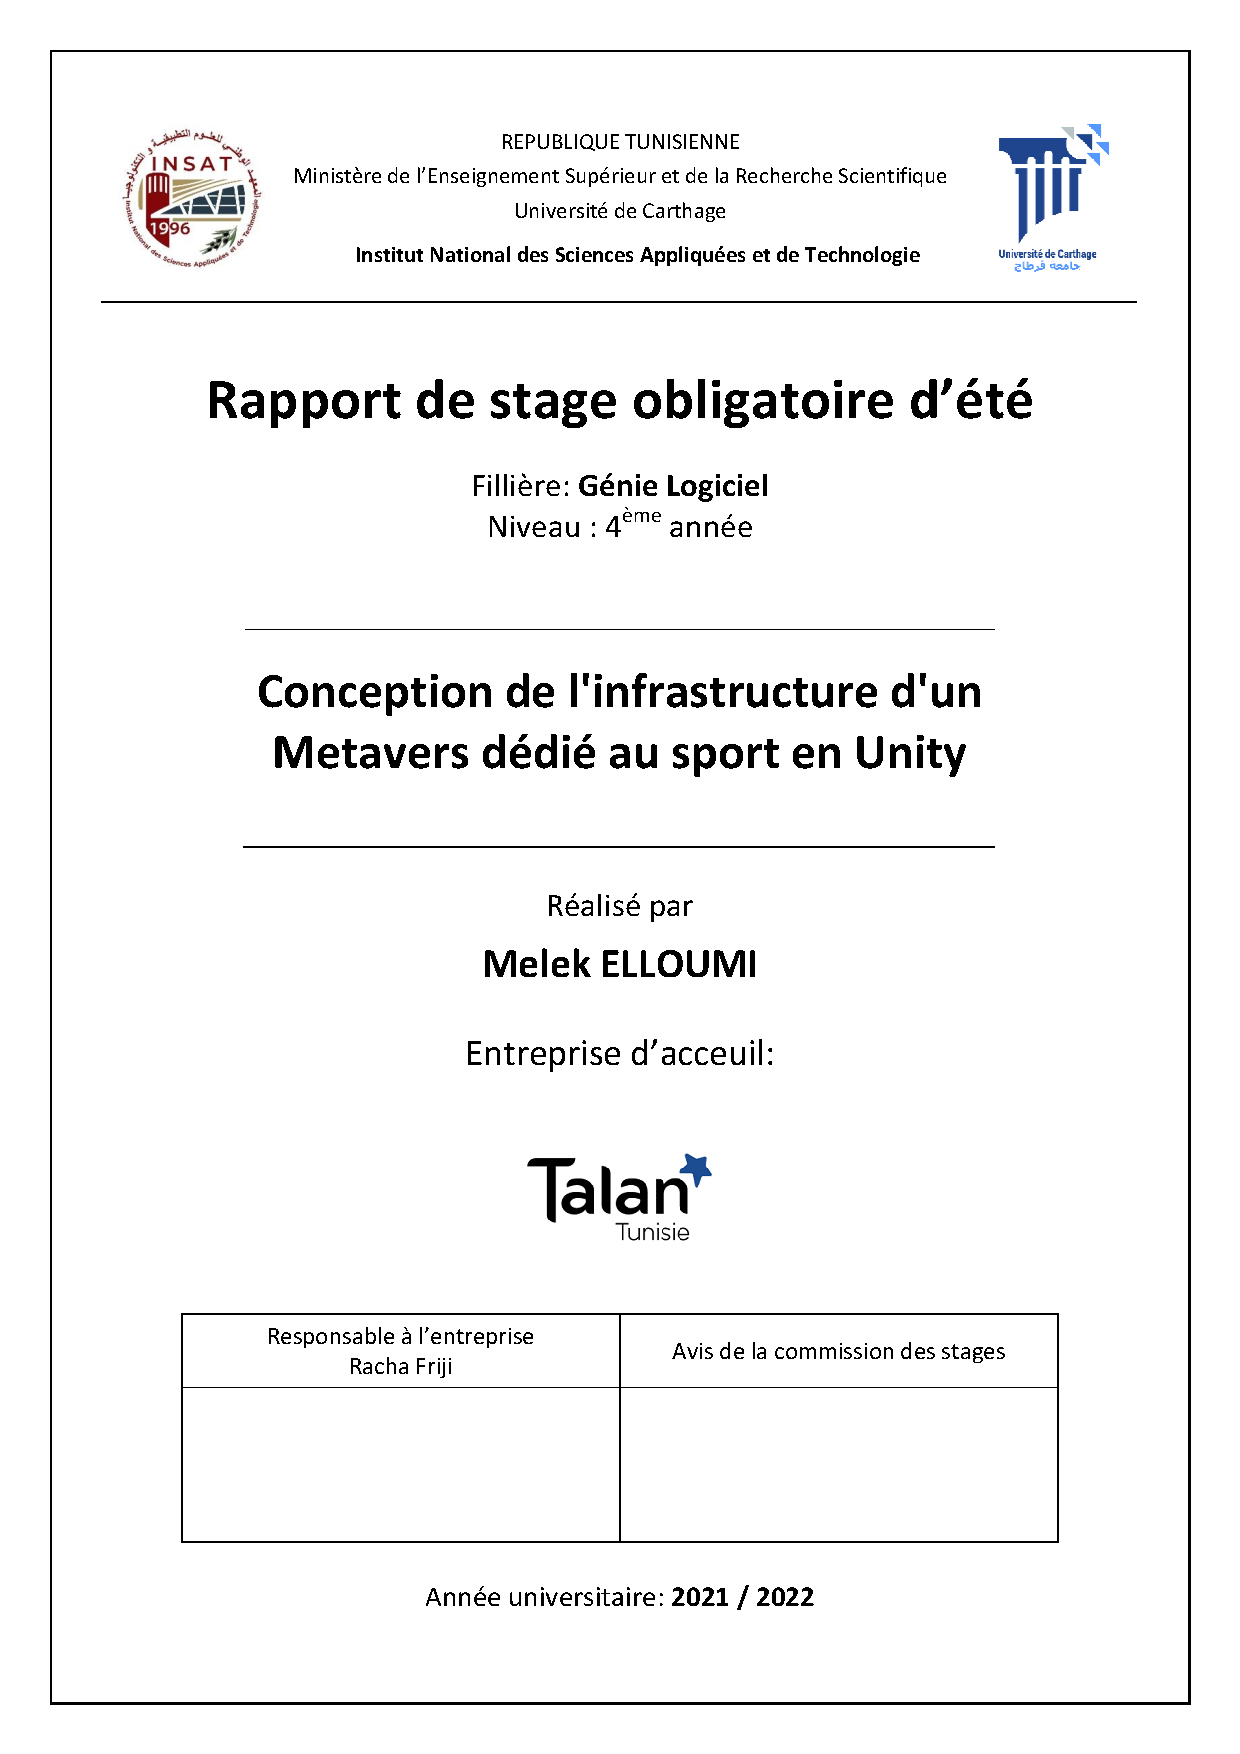
\includepdf[pages=-]{FrontPage.pdf}
\dominitoc
\mtcsettitle{minitoc}{Plan}
\mtcsetrules{*}{off}
\frontmatter
\spacing{1.4}
\afterpage{\blankpage}
\chapter*{\textbf{Remerciements}}
\normalsize{
\quad Nous tenons à exprimer notre gratitude à tous ceux qui nous ont aidés à atteindre cet objectif du projet.

\indent Je tiens à exprimer mes plus vifs remerciements à textbf{Mme Imen Ayari} et textbf{Mme Friji Racha}
pour leur encadrement tout au long du stage. Leur disponibilité, leur confiance et leurs conseils m’ont beaucoup aidé à atteindre les objectifs du projet dans les délais.

\indent Je tiens aussi à remercier toute l'équipe de l'Innovation Factory et Talan Tunisie pour cette magnifique opportunité et cette formation enrichissante.

\indent Je remercie également tous les professeurs de l'INSAT qui m'ont appris les bases de l'informatique tout au long de ces quatre années et pour les connaissances qu'ils m'ont transmises.
}


\spacing{0.9}

\tableofcontents
\newpage 
\listoffigures \mtcaddchapter 
\newpage 
\spacing{1.2}

\mainmatter
%\mtcaddchapter[Introduction générale] 
\chapter*{\textbf{Introduction générale}}
\addcontentsline{toc}{chapter}{Introduction générale}
\markboth{Introduction générale}{}

\lettrine[findent=2pt]{\textbf{A}}{ }près la pandémie de COVID-19, l'envie de virtualiser tous les aspects de la vie s'est encore accrue que jamais. C'est à ce moment que le métavers a été introduit. C'est un réseau persistant d'un monde virtuel interconnecté destiné à la communication en temps réel où les utilisateurs peuvent travailler, socialiser et faire des affaires, ou même jouer. L'utilisateur est complètement immergé dans l'environnement virtuel grâce à une virtualisation avancée.

C'est dans ce contexte que s'inscrit notre projet de stage dont l'objectif est de mettre en place un monde virtuel des jeux olympiques où l'utilisateur peut assister à des Coupes du monde, visiter des musées ou même des magasins pour acheter des produits virtuels. Il peut également interagir avec d'autres utilisateurs de n'importe quel pays par texte, audio et gestes. Notre équipe est responsable de concevoir l'infrastructure du projet pour intégrer le travail des autres équipes.


Notre rapport sera divisé en trois chapitres se terminant par une conclusion générale.

Le premier chapitre \textbf{« Contexte général »} est une présentation générale de notre travail dans lequel nous présentons l'organisation et le projet.

Le deuxième chapitre chapitre \textbf{« Spécification des besoins et plan »} identifie les exigences
de notre solution. Il contient les concepts de base que nous utilisons et le plan du deroulement du stage.

Le troisième chapitre \textbf{« Réalisation » } montre l'environnement utilisé pour l'implémentation de l'infrastructure du metavers et le travail réalisé.

\chapter{Contexte général}
\label{ch:1er}
\section*{Introduction}
Dans ce premier chapitre, nous nous concentrons d'abord sur le contexte général de notre projet. Nous commencerons avec une présentation de l'entreprise d'accueil. Puis, après avoir presenté le projet, nous allons
aborder l'étude de l'existant.

\section{Présentation de l'entreprise}
Cette section est dédiée à la présentation de l'organisation hôte ainsi que ses activités principales et ses domaines d'expertise.
\subsection{Talan Tunisie}
Talan \cite{talan} est un cabinet de conseil expert en transformation Agile. Créé en 2002 par Mehdi Houas, Eric Benamou et Philippe Cassoulat, Talan a réalisé en 2017 un chiffre d'affaires annuel de 185 millions d'euros. \newline L'entreprise propose son expertise métier et technologique à l'international, avec près de 2000 consultants partout dans le monde. Talan, acteur français majeur du Conseil aux Entreprises et en Informatique
monde, est basé à Paris et possède des bureaux à Aix-en-provence, Bordeaux, Lille, Lyon, Nantes,
Rennes, Toulouse, Belgique, Canada, Espagne, États-Unis, Luxembourg, Royaume-Uni, Suisse et Tunisie.
Pour accélérer son développement, Talan a lancé en 2008 un centre de développement nearshore à
la Tunisie qui s'appelle Talan Tunisie Consulting.

Les activités de Talan relèvent des secteurs présentés dans la \autoref{fig:talansec}.
\begin{figure}[H]
    \centering
    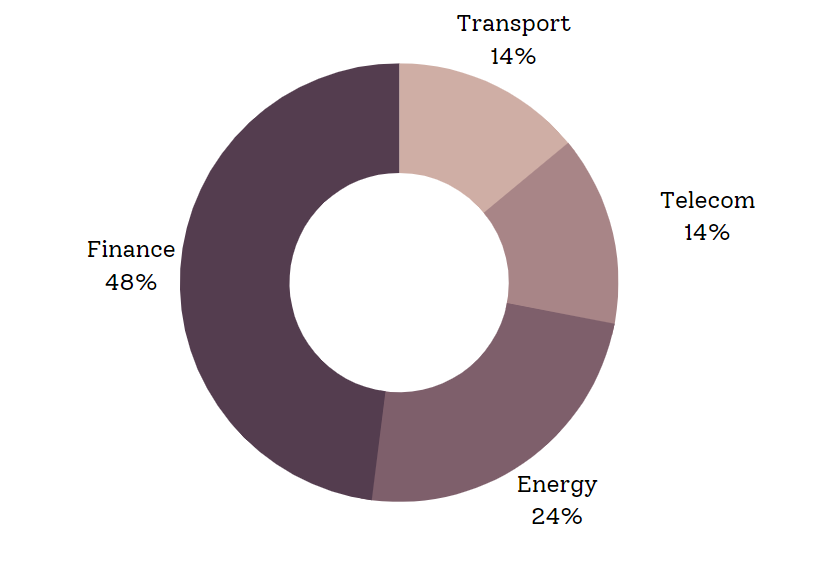
\includegraphics[width=0.6\textwidth]{figure/talansec.png}
    \caption{Répartition par secteur d'activité de Talan (2014)}
    \label{fig:talansec}
\end{figure}
\noindent

\subsection{Département Talan Innovation Factory}
Notre stage s'est déroulé au sein du département Innovation Factory de Talan Tunisie. Talan Innovation Factory représente le département recherche et développement de Talan qui explore et fournit une expertise relative aux technologies nouvelles et émergentes telles que la blockchain, le metavers, la réalité augmentée, la réalité mixte, et l'intelligence artificielle. \newline
De plus, ce département expérimente des méthodologies innovantes telles que la pensée et l'innovation Jugaad.


\section{Présentation du projet}
Plusieurs solution ont proposé diverses solutions à notre problème. Dans ce segment, nous
étudions trois projets existants, puis nous proposons notre propre solution selon nos besoins.
\subsection{Solutions existantes}
\subsubsection*{Decentraland}
Decentraland \cite{decentraland} est un monde virtuel basé sur Ethereum où l'utilisateur peut jouer, explorer,
et interagir avec des jeux et des activités. Il peut également acheter des parcelles de terrain sur lesquelles ils peuvent construire leurs propres environnements, places de marché et applications.

\begin{figure}[H]
    \centering
    
\includegraphics[width=0.6\textwidth]{figure/decentraland.png}
    \caption{Decentraland}
    \label{fig:decentraland}
\end{figure}
\noindent

\subsubsection*{The Sandbox}
Le Sandbox \cite{sandbox} est un monde virtuel décentralisé et communautaire où les créateurs peuvent
concevoir, partager et vendre des actifs dans le monde en utilisant le concept "jouer pour gagner". Il est unique dans le fait que tout object est construit à partir d'une particule cubique appelée "Voxel".
\begin{figure}[H]
    \centering
    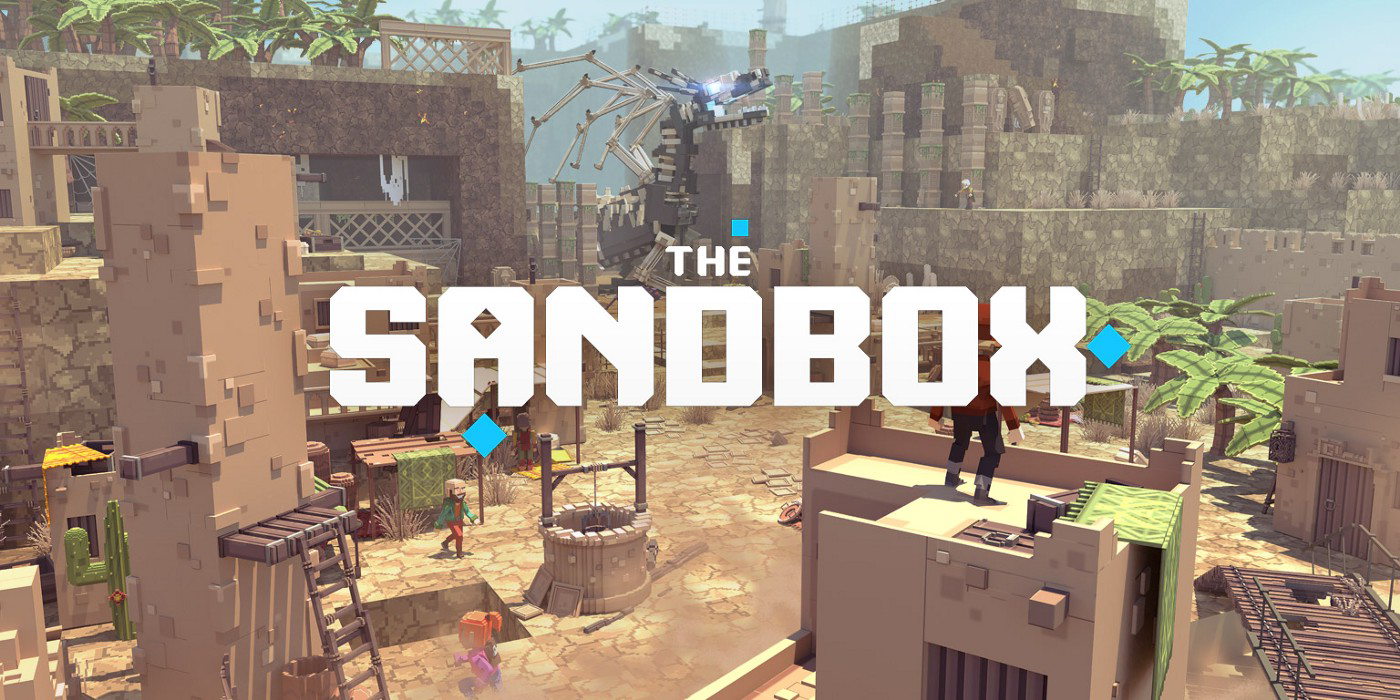
\includegraphics[width=0.6\textwidth]{figure/sandbox.png}
    \caption{The Sandbox}
    \label{fig:sandbox}
\end{figure}
\noindent

\subsubsection*{Meta-Talan}
MetaTalan \cite{talan} est une expérience immersive, où l'utilisateur vie l'expérience des travailleurs dans un
environnement de travail extraordinaire. Dans ce métavers, il peut parler à des collègues,
leur envoyer un message ou un e-mail.
Ce metavers est développé par l'équipe de Talan Innovation Factory en début 2022 en créant une version virtuelle du siège de Talan Tunisie, ce qui a permis de nous bien encadrer.
\begin{figure}[H]
    \centering
    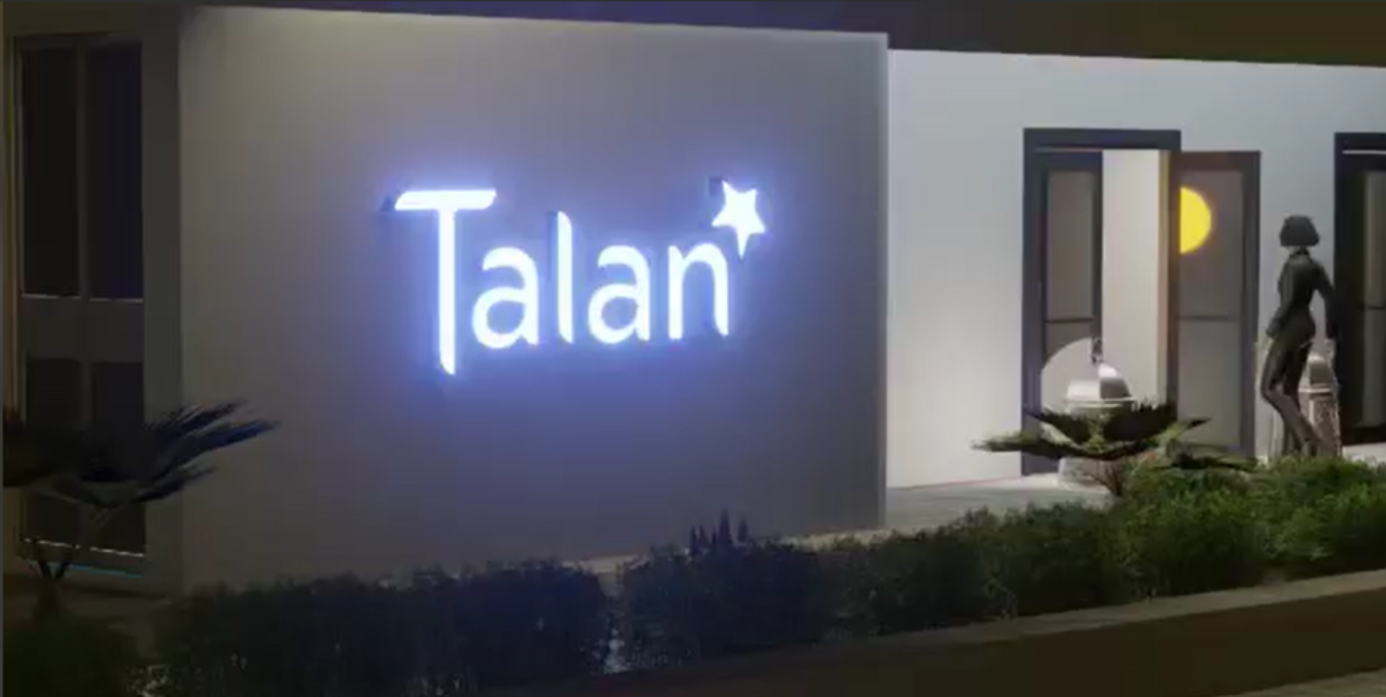
\includegraphics[width=0.6\textwidth]{figure/metatalan.png}
    \caption{Meta-Talan}
    \label{fig:metatalan}
\end{figure}
\noindent

\subsection{But du projet}
Le but de notre projet est d'implémenter un metaverse dans le domaine de sport. On veut prendre ce qui marche dans les plateformes existantes et les mettre dans notre projet qu'on a appelé MetaSport. Voici les besoins qu'on a planifier à mettre dans Metasport:
\begin{itemize}
\item[--] \textbf{Interactivité sociale entre utilisateurs :} chat vocal de proximité, système d’amis, gestes, éléments du monde interactifs, interface utilisateur intuitive.
\item[--] \textbf{Jeux de sport compétitifs :} Créer des jeux 3D et réalité mixte.
\item[--] \textbf{Place de marché décentralisée :} Crypto monnaie, NFTs d’accessoires de sport et d’avatar, billets d’événement.
\item[--] \textbf{Outils de création d’actifs :} donner aux utilisateurs les outils pour créer leurs propres actifs et les vendre dans les magasins.
\end{itemize}

\section*{Conclusion}
Dans ce chapitre, nous avons présenté Talan Tunisie et son département Talan Innovation Factory. Puis nous avons présenté les solutions metavers existants comme Decentraland, Sandbox et Meta-Talan. Enfin, on défniti le but de notre projet.


\chapter{Spécification des besoins et plan}
\label{ch:2eme}

\section*{Introduction}
Dans ce deuxième chapitre, nous nous détaillons les besoins de notre plateforme metavers et nous finirons par annoncer le plan choisi pour l'implementation tout au long du stage.

\section{Spécification et analyse des besoins}
Dans cette partie nous présentons l’analyse des besoins fonctionnels et non fonctionnels, ainsi
que les acteurs et les fonctionnalités de notre projet.
\subsection{Analyse des besoins}
\subsubsection*{Besoins fonctionnels}
Notre application doit répondre à l’ensemble des besoins fonctionnels suivants : 
\begin{itemize}
\item[--] L’utilisateur peut se connecter au metaverse avec un DAO unique.
\item[--] L’utilisateur peut interagir avec les autres utilisateurs avec un système de chat vocal ou de
chat textuel.
\item[--] L’utilisateur peut participer à des jeux sportifs multijoueurs par l’intermédiaire de portails
spéciaux.
\end{itemize}

\subsubsection*{Besoins non fonctionnels}
Les besoins non fonctionnels de notre application sont représentés ci-dessous :
\begin{itemize}
\item[--] \textbf{La sécurité :} on assure la sécurité des transactions par un réseau du blockchain qui
produit une structure de données avec des qualités de sécurité inhérente.
\item[--] \textbf{L’ergonomie et la convivialité :} L’application fournira une interface simple que son
utilisation ne nécessite aucun pré-requis afin d’assurer que les non-experts en informatique
peuvent l’utiliser.
\item[--] \textbf{L’extensibilité et maintenabilité :} L’architecture de l’application permettra la maintenance
et l’évolution au niveau du projet.
\item[--] \textbf{Disponibilité :} L’application doit être toujours disponible même pendant la période de
maintenance.
\end{itemize}

\subsection{Spécification des besoins}
Dans cette partie, on va mieux présenter les spécifications du projet. On a choisi le diagramme de cas d’utilisation et le diagramme de séquence afin de bien expliquer les fonctionnalités
de notre application.

\subsubsection*{Diagramme de cas d’utilisation}
Le diagramme de cas d’utilisation présenté dans la \autoref{fig:usecase} montre l’acteur et ses
interactions principales avec l’application.

\begin{figure}[H]
    \centering
    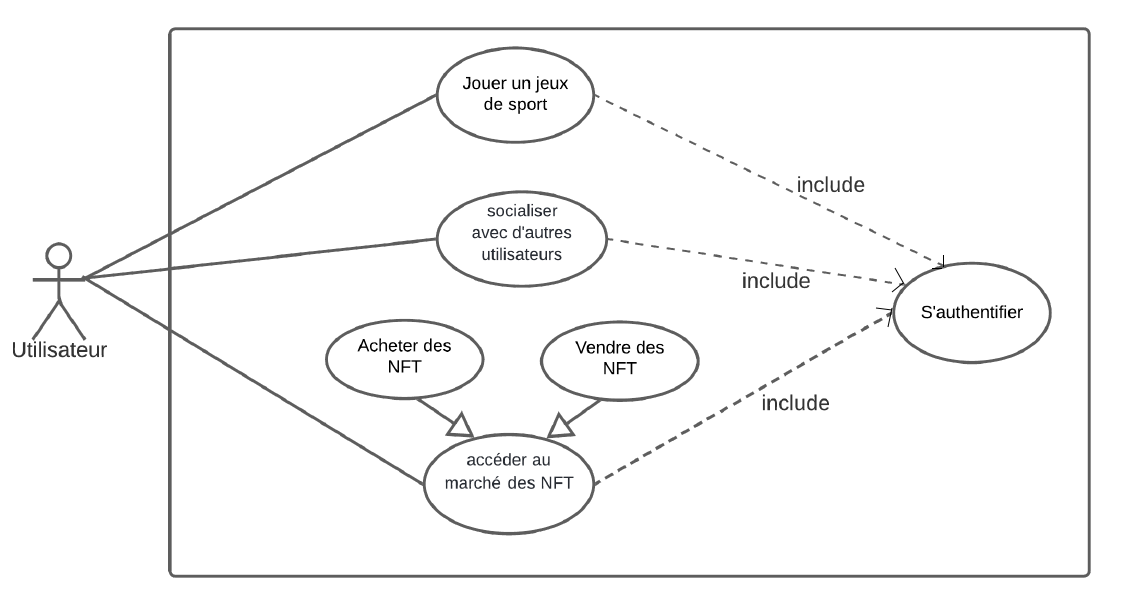
\includegraphics[width=0.7\textwidth]{figure/usecase.png}
    \caption{Diagramme de cas d’utilisation}
    \label{fig:usecase}
\end{figure}
\noindent

\subsubsection*{Diagramme de séquence système}
La \autoref{fig:sequence} présente le diagramme de séquence système de l'action "Registrer" de notre application pour un simple utilisateur.

\begin{figure}[H]
    \centering
    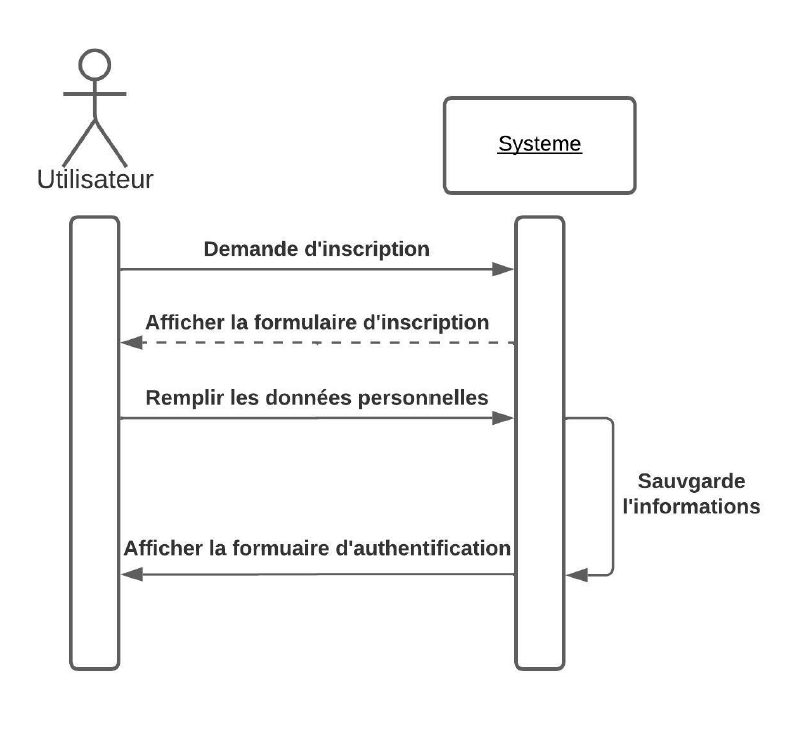
\includegraphics[width=0.4\textwidth]{figure/sequence.png}
    \caption{Diagramme de séquence - Registrer}
    \label{fig:sequence}
\end{figure}
\noindent


\section{Plan}
Dans cette partie nous présentons la méthode de travail et les technologies qu'on a choisies ainsi que le déroulement du stage.
\subsection{Méthode de travail}
Après avoir étudié les exigences et les objectifs du projet, il est crucial d’adopter une méthodologie de gestion de projet afin de mieux répondre aux exigences de notre projet et de le réussir.
Basé sur la nature de notre projet, nous avons adopté la méthodologie Agile.

\noindent
Le travail est divisé en de multiples petits sprints avec des différents buts. Ils ont duré une semaine en moyenne. Nous avons aussi divisé les stagiaires en six équipes de rôles différents. Cette méthode nous a permis de bien diviser les tâches, amplifier l'acquisition des informations et accélerer l'implementation du prototype finale.

\noindent
Le plan est de former les stagiaires dans les technologies du metavers, faire une synthèse sur les plateformes de metavers existantes et enfin passer à l'implementation de notre projet Metasport avec une vision commune entre les équipes. Je suis dans l'équipe "Tankers" dont le rôle est la conception de l'infrastructure du projet en Unity pour l'intégration des travaux des autres équipes.

\subsection{Technologies choisies}
Pour implémenter le monde virtuel d'un metavers, on devait chercher et comparer les outils de développement 3D. On a donc décidé de travailler avec ces ressources:

\subsubsection*{Unity}
Unity \cite{unity} est un moteur de jeu multiplateforme développé par Unity Technologies, il peut être utilisé pour créer
des jeux tridimensionnels (3D) et bidimensionnels (2D), ainsi que des simulations interactives et
d'autres expériences.
\begin{figure}[H]
    \centering
    
\includegraphics[width=0.25\textwidth]{figure/unity.png}
    \caption{Logo de Unity}
    \label{fig:unity}
\end{figure}
\noindent

\subsubsection*{Photon}
Photon Unity Networking (PUN) \cite{Photon} est un package Unity pour les jeux multijoueurs. Sa mise en relation flexible
amène les joueurs dans des lieux où les objets peuvent être synchronisés sur le réseau.
\begin{figure}[H]
    \centering
    
\includegraphics[width=0.25\textwidth]{figure/photon.png}
    \caption{Logo de Photon}
    \label{fig:photon}
\end{figure}
\noindent

\subsubsection*{Blender}
Blender \cite{blender} est un ensemble d'outils logiciels d'infographie 3D gratuits et open-source utilisés pour créer les
films d'animation, les effets visuels, les modèles imprimés en 3D,  les animations graphiques et les jeux vidéo.
\begin{figure}[H]
    \centering
    
\includegraphics[width=0.25\textwidth]{figure/blender.png}
    \caption{Logo de Blender}
    \label{fig:blender}
\end{figure}
\noindent
\newpage
\subsection{Journal de stage}
La \autoref{fig:gantt} présente le diagramme de Gantt qui résume les étapes qu'on a pris afin de réaliser MetaSport dans les 2 mois de Juillet et Août 2022.
\begin{figure}[H]
    \centering
    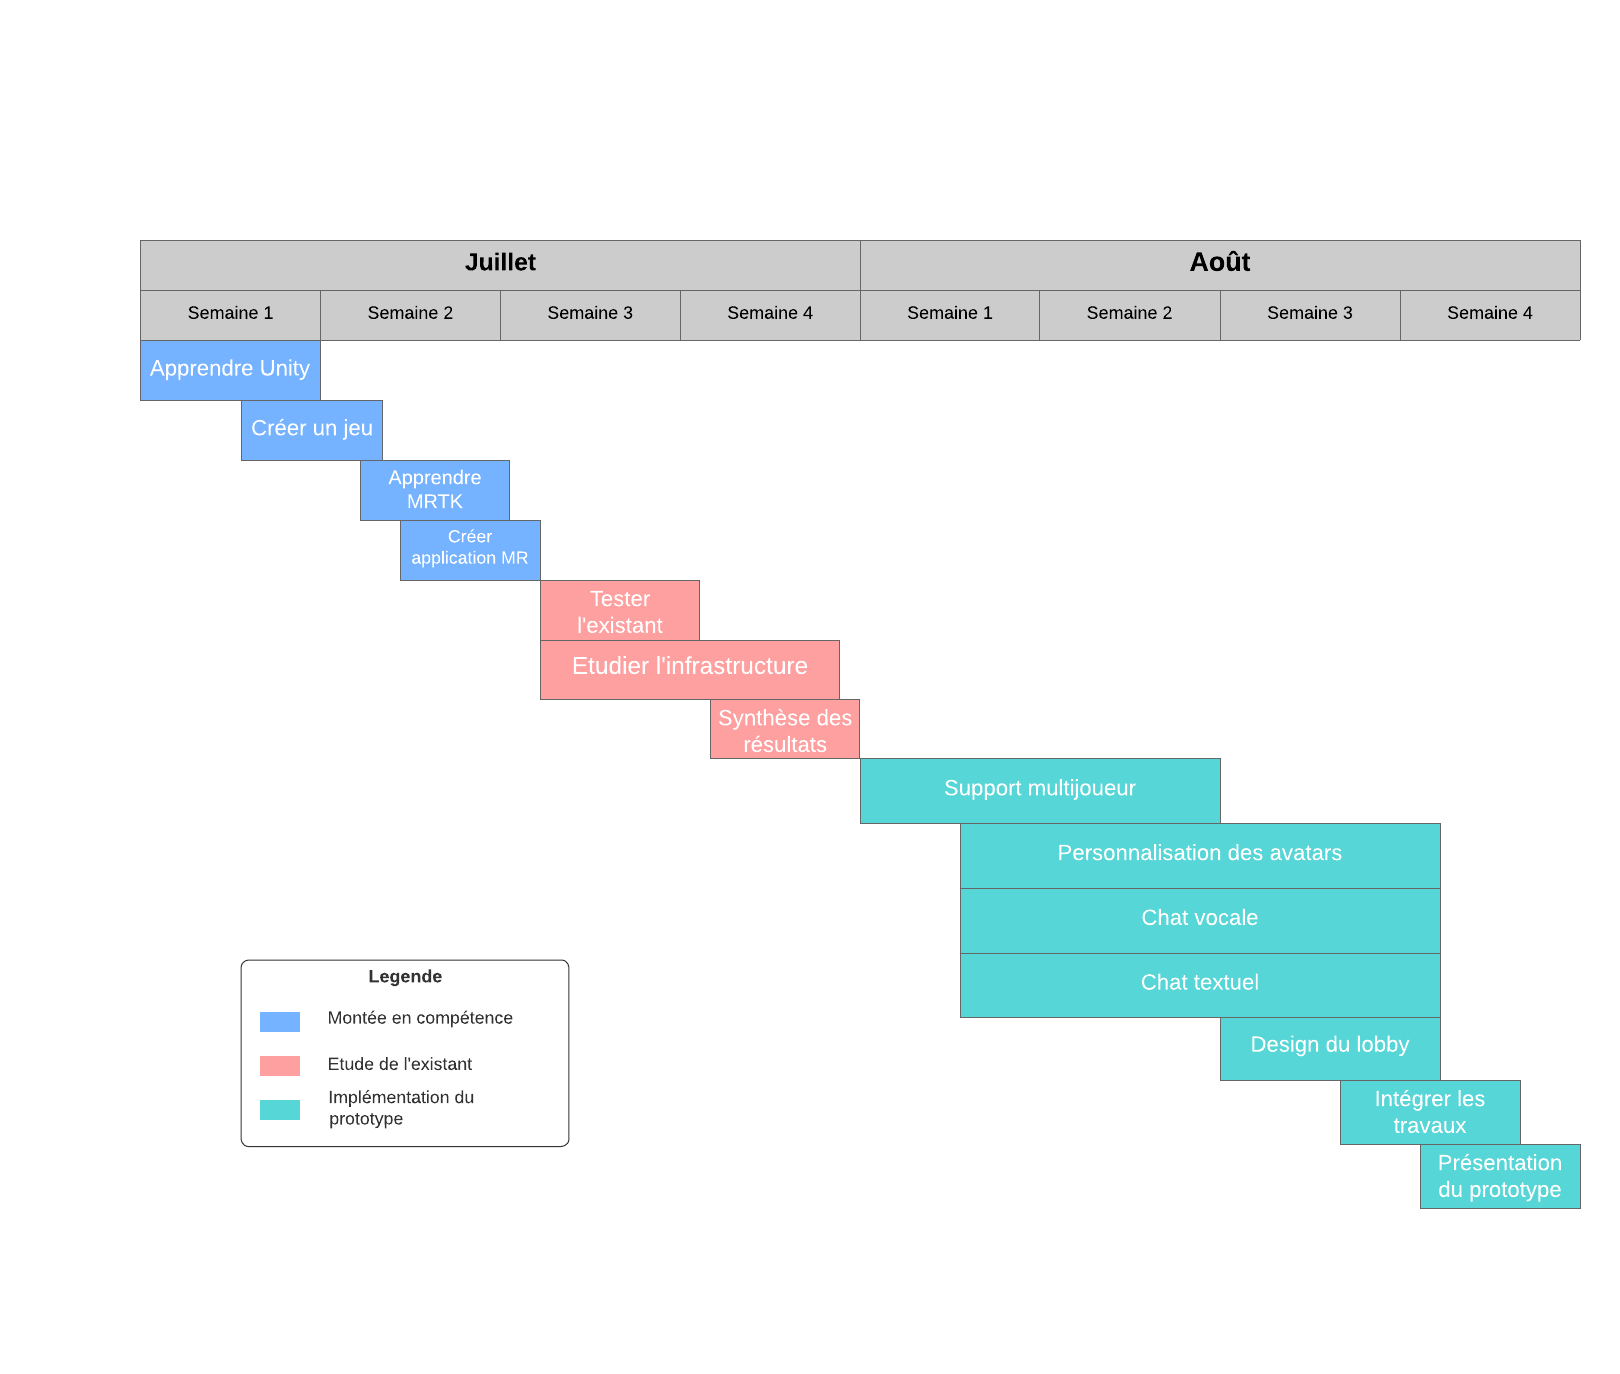
\includegraphics[width=0.75\textwidth]{figure/gantt.png}
    \caption{Diagramme de Gantt du stage}
    \label{fig:gantt}
\end{figure}
\noindent

\section*{Conclusion}
Dans ce chapitre, nous avons décomposé l’analyse des besoins en deux catégories : les besoins fonctionnels et les besoins non fonctionnels. Puis nous avons présenté les schémas qui montrent le fonctionnement principal du système. Enfin, on termine par le plan. Dans le prochain chapitre, nous aborderons la phase de réalisation.



\chapter{Réalisation}
\label{ch:3eme}

\section*{Introduction}
Dans ce dernier chapitre, nous nous concentrons d'abord sur l'environnement de travail. Puis, nous présentons des captures du travail réalisé et les acquis du stage.
\section{Environnement de travail}
Cette section présente les outils de développement matériel et logiciel de notre projet en tenant
compte de leur utilisation importante.
\subsection{Environnement matériel}
Voici l’environnement matériel sur lequel nous avons intégré notre projet :
\begin{itemize}
\item[--] \textbf{Marque :} MSI
\item[--] \textbf{Processeur :} Intel Core i7-9750H
\item[--] \textbf{Mémoire :} 16 GB RAM
\item[--] \textbf{Carte Graphique :} Nvidia GeForce RTX 2060
\item[--] \textbf{Système d'execution :} Windows 10
\end{itemize}

\subsection{Environnement logiciel}
Dans cette partie nous allons citer les outils logiciels utilisés dans le développement de ce projet :
\begin{itemize}
\item[--] \textbf{Microsoft Visual Studio 2022 :} est un environnement complet de codage, principalement en C\#.
\item[--] \textbf{Unity :} Unity3D est un moteur de jeu qui peut être utilisé pour développer des jeux vidéo pour PC, consoles, appareils mobiles et sites Web.
\item[--] \textbf{Blender:} est un logiciel open source de modélisation, d’animation et de creation d'objets 3D.
\item[--] \textbf{GitHub :} est un service d’hébergement de référentiel Git, mais il ajoute de nombreuses fonctionnalités spécifiques.
\end{itemize}

\section{Travail réalisé}
Dans cette partie, nous vous présentons des captures d’écran du métavers réalisé chaque image
affiche une partie de l’espace créé.
\noindent
Cette première interface d’authentification où l’utilisateur peut créer son compte en donnant les
informations requises, puis il peut se connecter.
\begin{figure}[H]
    \centering
    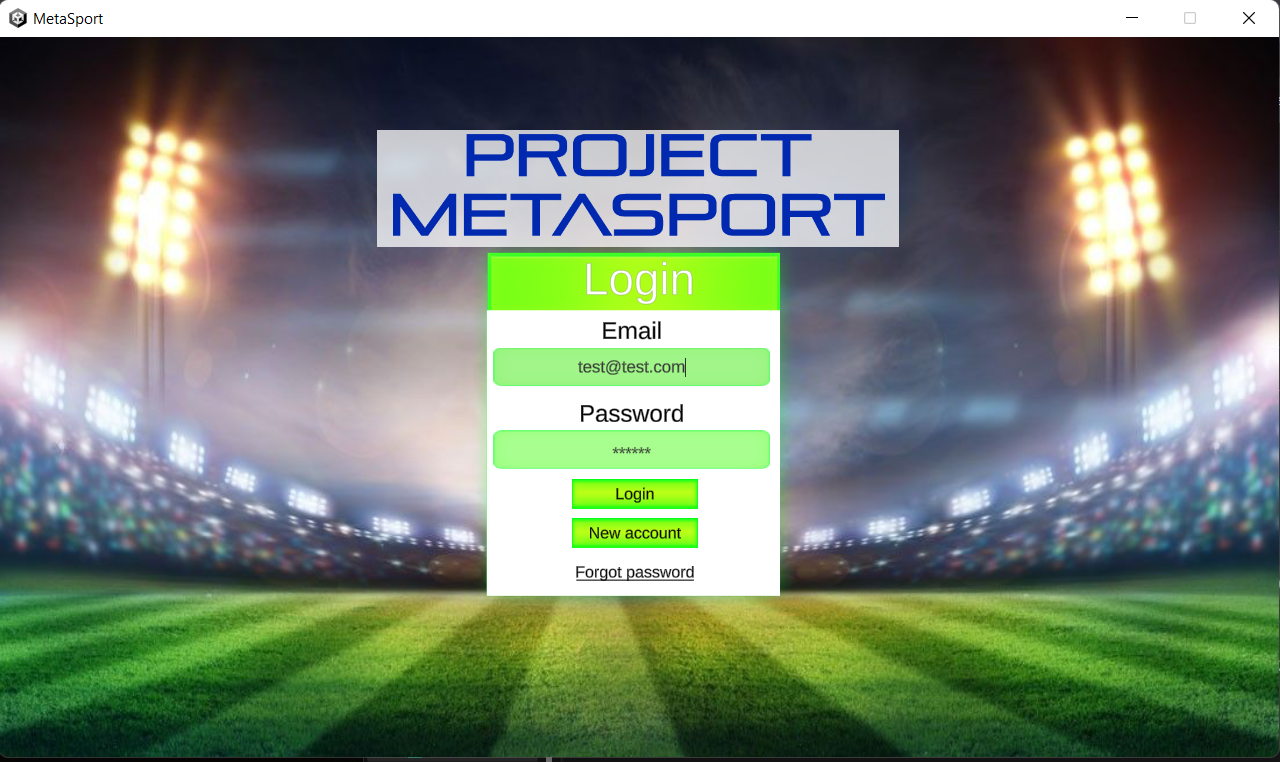
\includegraphics[width=0.65\textwidth]{figure/login.png}
    \caption{L’interface de l’authentification}
    \label{fig:login}
\end{figure}
\noindent

Dans cette figure nous montrons le système de création de l’avatar, c’est le personnage qui
représente l'utilisateur dans les métavers. Il peut choisir ses vêtements et personnaliser son look.
\begin{figure}[H]
    \centering
    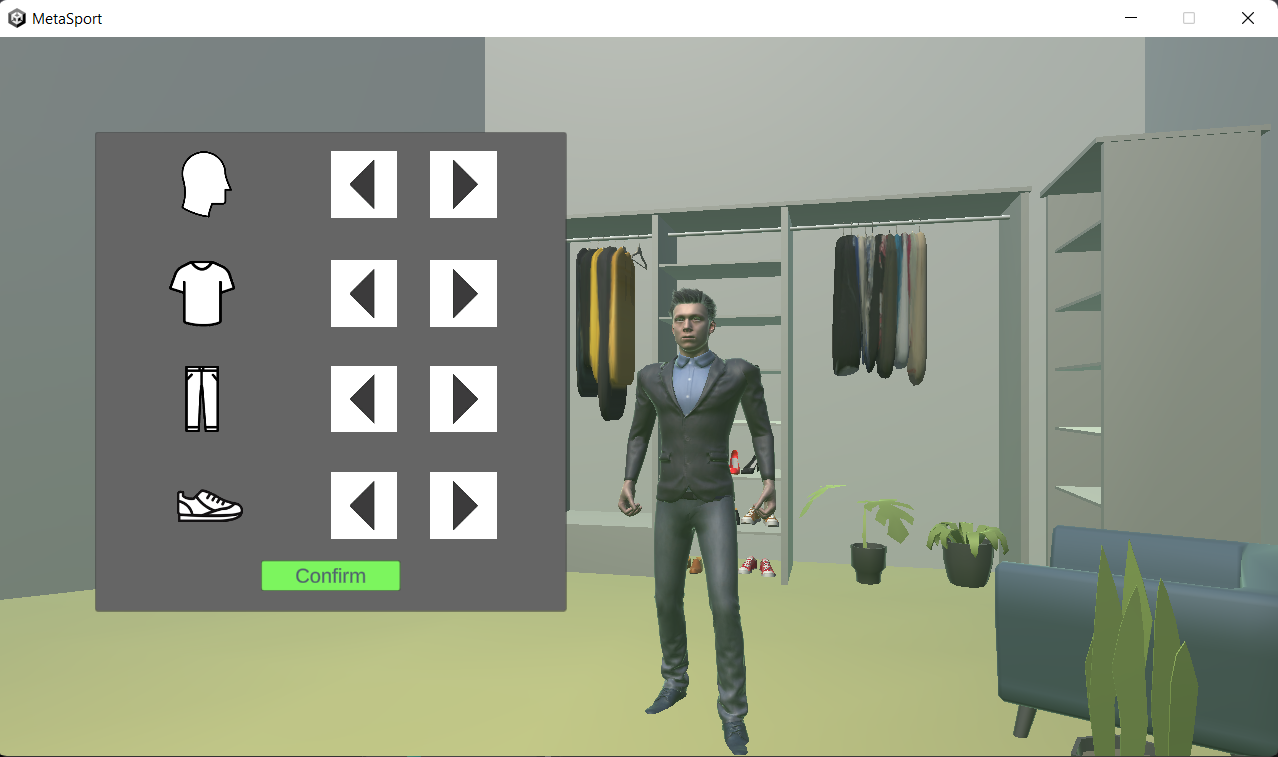
\includegraphics[width=0.65\textwidth]{figure/char.png}
    \caption{Selection de l'avatar}
    \label{fig:char}
\end{figure}
\noindent

Après l’authentification, les utilisateurs apparaissent dans une zone commune, c’est le "lobby" où ils peuvent interagir et communiquer.
\begin{figure}[H]
    \centering
    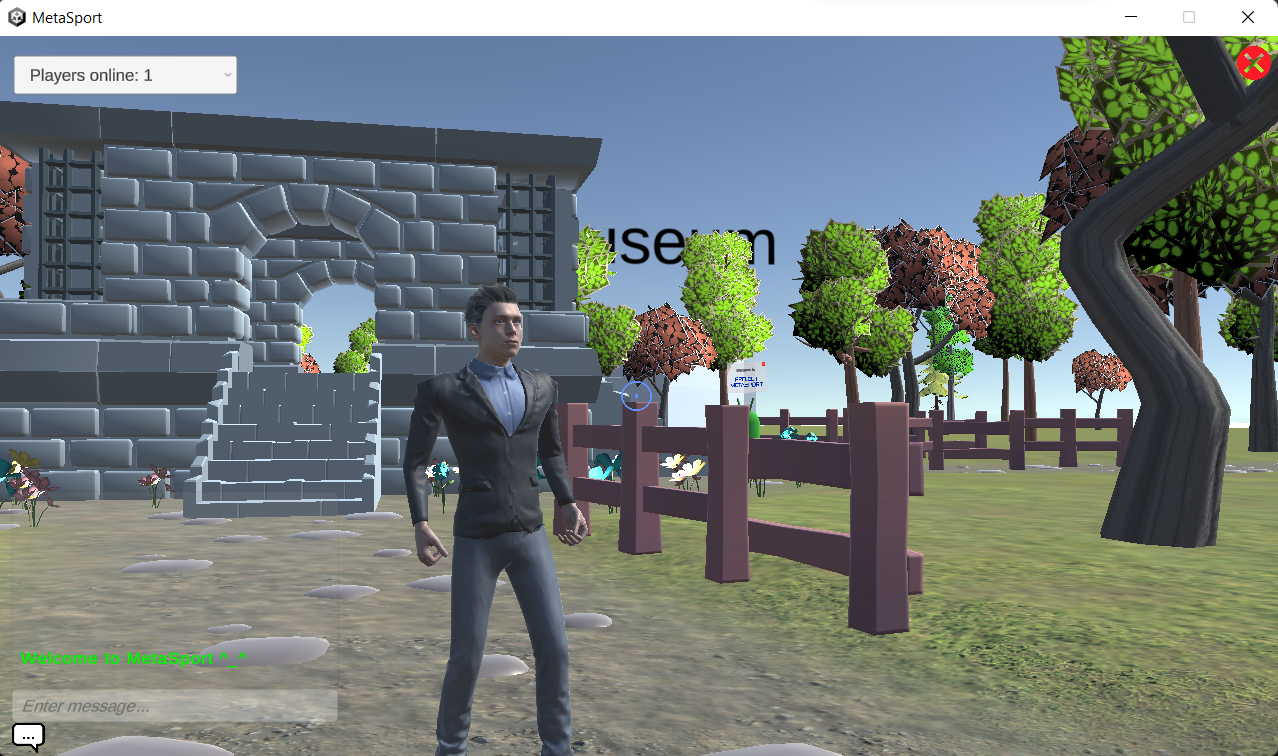
\includegraphics[width=0.65\textwidth]{figure/lobby.png}
    \caption{Le lobby où les joueurs apparaissent}
    \label{fig:lobby}
\end{figure}
\noindent

Dans la \autoref{fig:chat}, on peut voir la fonctionnalité de chat textuel où les utilisateurs peuvent écrire des messages publiques et privés.
\begin{figure}[H]
    \centering
    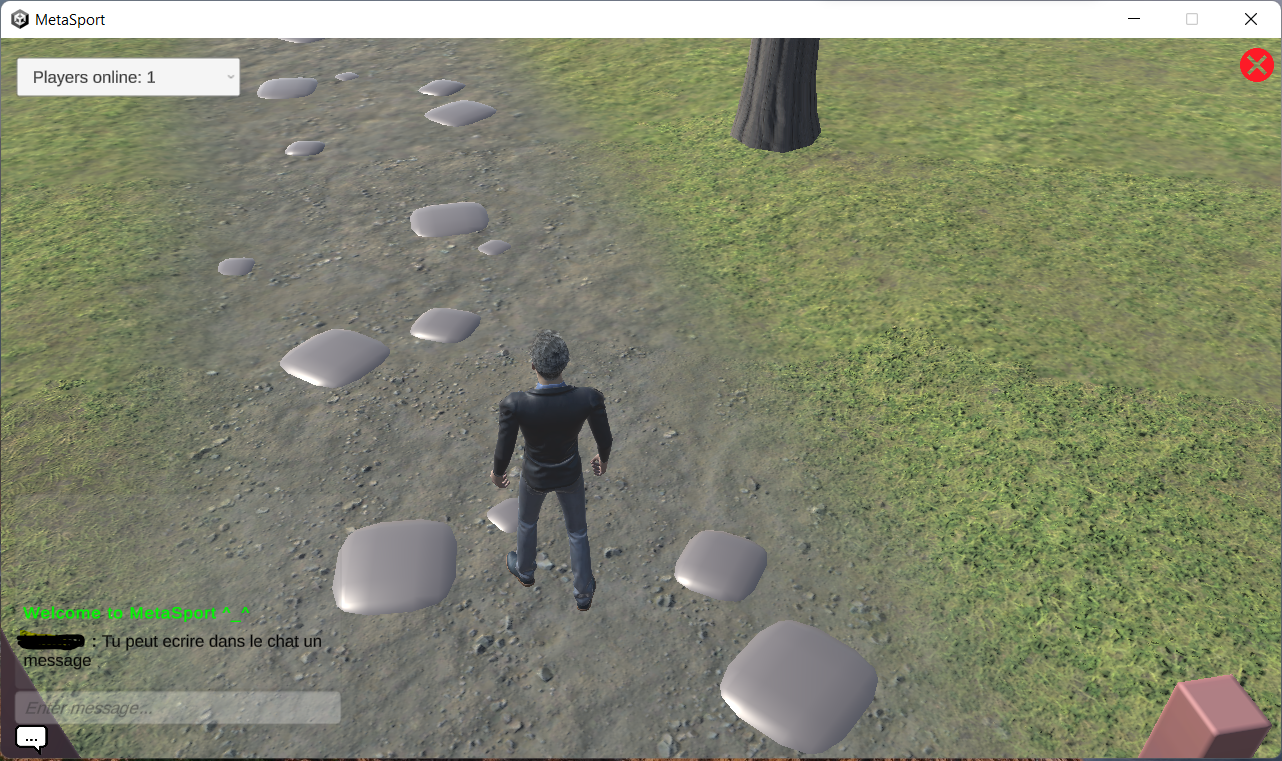
\includegraphics[width=0.6\textwidth]{figure/chat.png}
    \caption{L’utilisation de chat pour la communication}
    \label{fig:chat}
\end{figure}
\noindent

La \autoref{fig:inUnity} montre l'envirennoment de développement Unity.
\begin{figure}[H]
    \centering
    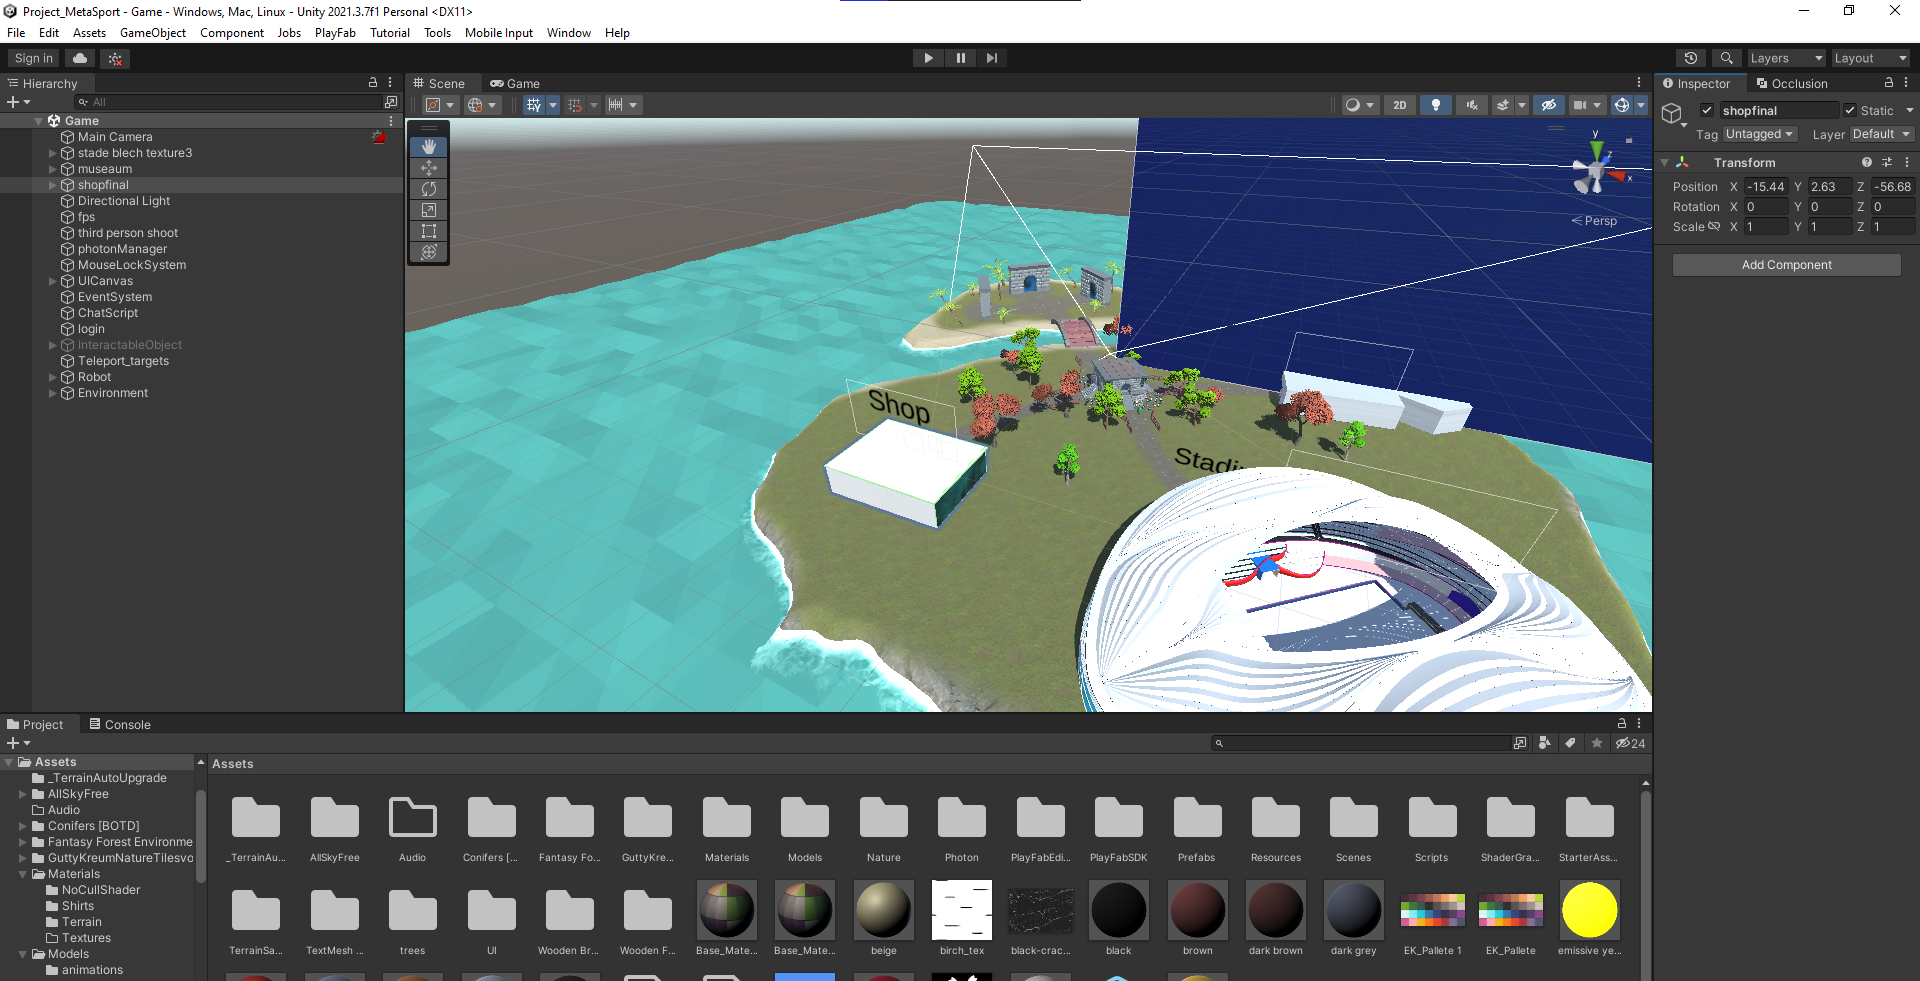
\includegraphics[width=0.65\textwidth]{figure/inUnity.png}
    \caption{L’interface de l’authentification}
    \label{fig:inUnity}
\end{figure}
\noindent



\section{Consolidation des acquis}
Ce tableau résume les compétences que j'ai utilisé dans ce stage d'été dont j'ai appris dans ma formation à l'INSAT.
\begin{table}[H]
\label{tab:acquis}
\centering
\renewcommand{\arraystretch}{1.65}
\begin{tabular}{| C{.5\textwidth} | C{.5\textwidth} |} 
\hline
\textbf{Cours enseigné à l'INSAT} & \textbf{Compétence aquise} \\ 
\hline 
\hline 
Design patterns & Optimisation des classes \\ 
\hline 
Complexité & Optimisation des algorithmes \\ 
\hline 
Fondament des systèmes repartis & Conception du système multijoueur \\ 
\hline 
Méthodologie agile & Méthodologie de travail dans l'entreprise \\ 
\hline 
Qualité & Clean code \\ 
\hline 
GRH & Management d'une petite équipe \\ 
\hline 
IHM & Ergonomie \\ 
\hline 
\end{tabular}
\end{table}


\section*{Conclusion}
Dans ce chapitre, nous avons indiqué l'utilissation d'un ordinateur puissant avec plusieurs logiciels pour développer MetaSport. Nous avons aussi montrer quelques images de l'execution de l'application. Ma formation à l'INSAT m'a aidé enormément dans ce stage et je trouve que je suis compétent.

\chapter*{\textbf{Conclusion et perspectives}}
\addcontentsline{toc}{chapter}{Conclusion et perspectives}
\markboth{Conclusion et perspectives}{}
\lettrine[findent=2pt]{\textbf{D}}{ }ans le cadre du stage d’été avec Talan Tunisie, il nous a été demandé de développer un metavers
dédié au sport. Dans ce metavers, l’utilisateur est présenté par un espace où il peut intéragir avec d’autres utilisateurs avec un systeme de chat textuel et vocale. En plus, on a developpé trois jeux de sport que l’utilisateur peut jouer en multijoueur.

Dans ce rapport, nous avons présenté les différentes étapes menantes à la réalisation de ce projet
en trois parties. Dans la première partie, nous avons commencé par une présentation générale. L’étude des solutions existantes pour les améliorer et nous avons présenté Talan Tunisie et son département hôte.
Dans la deuxième partie, nous avons précisé les besoins et identifié les fonctionnalités que l’application devait atteindre, puis nous avons détaillé le plan de travail.
Enfin, dans le dernier chapitre, nous avons expliqué la mise en
oeuvre en présentant l’environnement de travail et les résultats avec des captures d’écran.

Lors de la mise en place de ce projet, nous avons rencontré quelques difficultés alors que nous
assemblions les différentes parties du projet sur un seul PC. Ces difficultés sont l’incompatibilité de
certaines parties du code avec d’autres parties qui proviennent des autres équipes qui n'ont pas respecter les conventions d'optimisation, et la manque de puissance de l'ordinateur dans le rendement des objets.

Dans une optique d’amélioration continue, nous prévoyons :
\begin{itemize}
\item[--] D'ajouter un chatbot pour améliorer l’intégration des nouveaux utilisateurs avec l’espace metavers.
\item[--] D'optimiser les objets 3D pour diminuer les erreurs techniques dans les PC faibles.
\item[--] De completer l’integration des différents jeux du sport au metavers.
\end{itemize}
\spacing{1.1}
\begin{flushleft}
    \bibliographystyle{unsrt}
    \bibliography{references}
\end{flushleft}

\end{document}